\actTitle{3.2 - Exponential Functions}

\videoLink{Section 3.2}{https://www.youtube.com/playlist?list=PLYHZK3b8UFw3OE2GrAT4IExxBw5meagdH}

\noindent \textbf{Topics:}  exponential functions, compound interest, the number $e$, exponential functions with base $e$, growth and decay\\

\noindent \textbf{Student Learning Outcomes:}
\begin{enumerate}
\item Students will be able to recognize an exponential function graphically and algebraically.
\item Students will be able to evaluate the exponential function base $e$.
\item Students will be able to use exponential functions in compound interest and growth/decay problems.
\end{enumerate}

\hrule 

\bigskip

\subsection{Exponential Functions} ~

\noindent\underline{Exponential functions $y=a^x$} (always assume $a>0$) \\[.2in]

  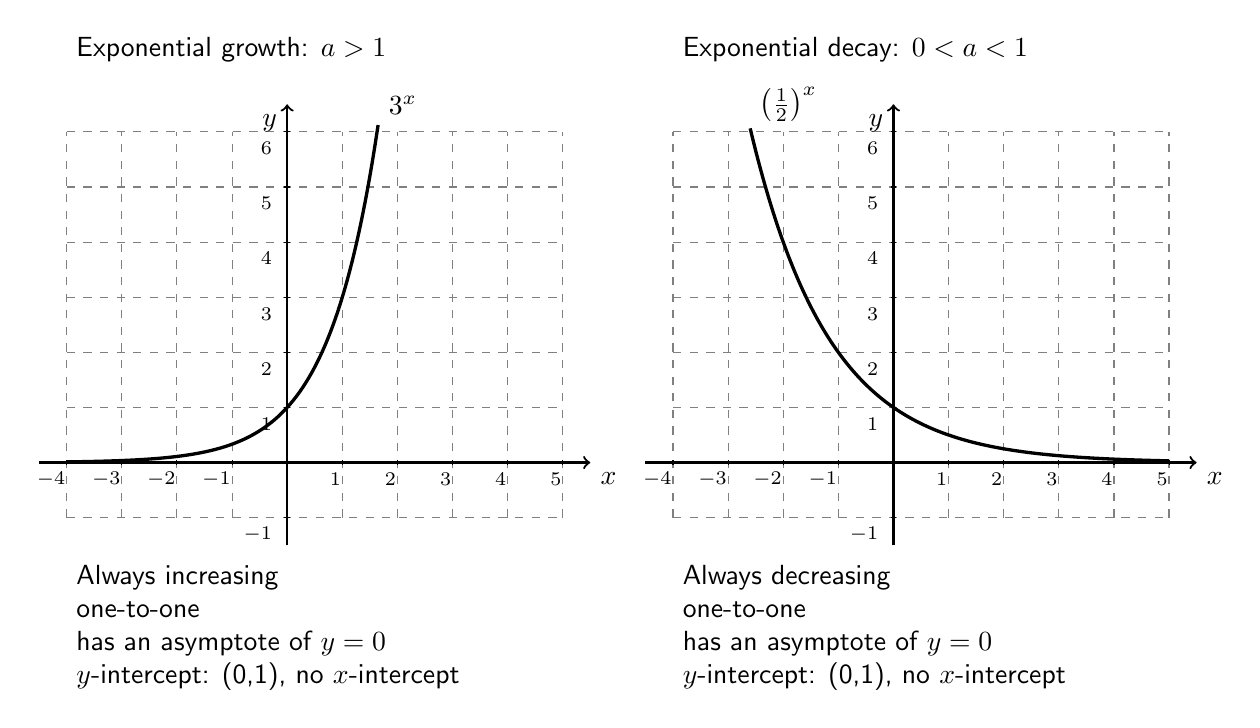
\begin{tikzpicture}[y=0.7cm, x=0.7cm,font=\sffamily]
    \begin{scope}
      %% ticks
      \draw[step = 1.0, gray,dashed] (-4,-1) grid (5,6);
      %% axis
      \draw[thick,->] (-4.5,0) -- coordinate (x axis mid) (5.5,0)
      node[anchor = north west] {$x$}; \draw[thick,->] (0,-1.5) --
      coordinate (y axis mid) (0,6.5) node[anchor = north east] {$y$};
      \foreach \y in {-1,1,2,3,4,5,6} { \draw (1pt, \y) -- (-1pt, \y)
        node[font=\scriptsize,yshift=-6,xshift=-1,anchor=east] {$\y$}; }
      \foreach \x in {-4,-3,-2,-1,1,2,3,4,5} { \draw (\x,1pt) --
        (\x,-1pt) node[font=\scriptsize,yshift=-5,xshift=3,anchor=east]
        {$\x$}; }

      \node[anchor=west,align=left] at (-4,7.5) {Exponential growth: $a>1$};
      \node[anchor=west,align=left] at (-4,-3)
      {
        Always increasing \\
        one-to-one \\
        has an asymptote of $y=0$ \\
        $y$-intercept: (0,1), no $x$-intercept
      };
      
      \begin{scope}
        %% \clip(-4,-1) rectangle (8,5);
        \draw[scale=1.0,domain=-4:1.65,smooth,variable=\x,very
        thick,black,samples=100] plot ({\x},{3^\x}) node[anchor=south
        west] {$3^x$};
        %% \fill[black] (1/6,5) circle [radius=0.5ex] node[anchor=south
        %% west,xshift=-8] {$\left(\frac{1}{6},5\right)$};
      \end{scope}
     \end{scope}

     \begin{scope}[shift={(11,0)}]
      %% ticks
      \draw[step = 1.0, gray,dashed] (-4,-1) grid (5,6);
      %% axis
      \draw[thick,->] (-4.5,0) -- coordinate (x axis mid) (5.5,0)
      node[anchor = north west] {$x$}; \draw[thick,->] (0,-1.5) --
      coordinate (y axis mid) (0,6.5) node[anchor = north east] {$y$};
      \foreach \y in {-1,1,2,3,4,5,6} { \draw (1pt, \y) -- (-1pt, \y)
        node[font=\scriptsize,yshift=-6,xshift=-1,anchor=east] {$\y$}; }
      \foreach \x in {-4,-3,-2,-1,1,2,3,4,5} { \draw (\x,1pt) --
        (\x,-1pt) node[font=\scriptsize,yshift=-5,xshift=3,anchor=east]{$\x$};
      }

      \node[anchor=west,align=left] at (-4,7.5) {Exponential decay: $0<a<1$};
      \node[anchor=west,align=left] at (-4,-3)
      {
        Always decreasing \\
        one-to-one \\
        has an asymptote of $y=0$ \\
        $y$-intercept: (0,1), no $x$-intercept
      };

      \begin{scope}
        %% \clip(-4,-1) rectangle (8,5);
        \draw[scale=1.0,domain=-2.6:5,smooth,variable=\x,very thick,black,samples=100]
                 plot ({\x},{0.5^\x});
        \node[anchor=south west] at (-2.6,6) {$\left(\frac{1}{2}\right)^x$};
        %% \fill[black] (1/6,5) circle [radius=0.5ex] node[anchor=south
        %% west,xshift=-8] {$\left(\frac{1}{6},5\right)$};
      \end{scope}
     \end{scope}
   \end{tikzpicture}

\begin{eqnarray*}
  \begin{array}{rcl@{\hspace{4em}}rcl@{\hspace{4em}}rcl@{\hspace{4em}}rcl}
    f(x) & = & 2^x, & g(x) & = & 10^x, & h(x)&=&3^{x+1}, & j(x)&=&\left(\frac{1}{2}\right)^{x-1}. \\ [5pt]
    \multicolumn{3}{c}{\textrm{Base~is~2.}} &
    \multicolumn{3}{c}{\textrm{Base~is~10.}} &
    \multicolumn{3}{c}{\textrm{Base~is~3.}} &
    \multicolumn{3}{c}{\textrm{Base~is~}\frac{1}{2}.} 
  \end{array}
\end{eqnarray*}


\begin{enumerate}

\item Is $f(x)=1^x$ an exponential function?\\[.5in]



\item Is $f(x)=(-4)^x$ an exponential function?\\


\newpage
\item Graph $f(x)=3^{x-2}+4.$

      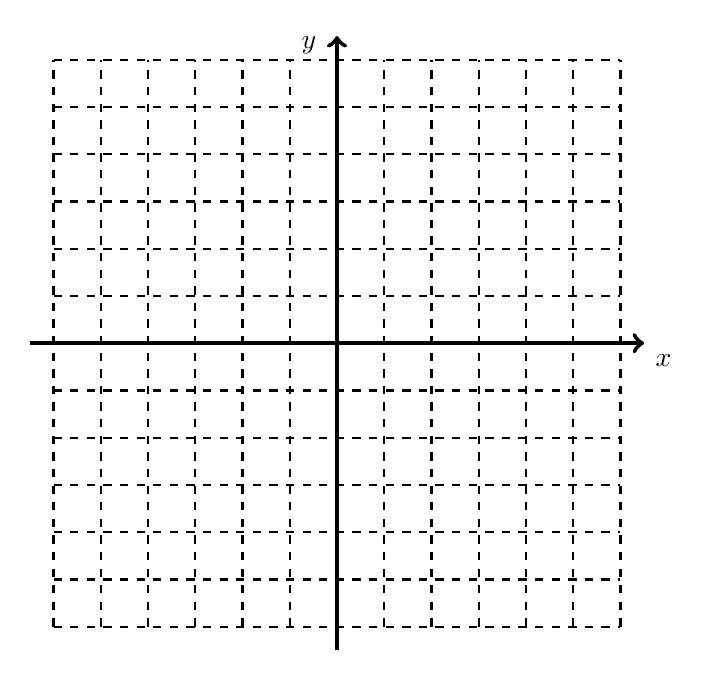
\begin{tikzpicture}[y=0.6cm, x=0.6cm,font=\sffamily]
        \begin{scope} %[shift={(0,8)}]
          %% ticks
          \draw[xstep = 1, ystep=1.0,black,dashed,thick] % very thin,opacity=0.85,
                 (-6.0,-6.0) grid ( 6.0, 6.0);
             %% axis
           \draw[ultra thick,->] (-6.5,0) -- coordinate (x axis mid) (6.5,0)
                node[anchor = north west] {$x$}; 
           \draw[ultra thick,->] (0,-6.5) -- coordinate (y axis mid) (0,6.5) 
                node[anchor = east,shift={(-0.2,-0.2)}]  {$y$};

           %\foreach \y in {-1,1,...,4} {
           %   \draw (1pt, \y) -- (-1pt, \y) node[yshift=-6,xshift=1,anchor=west] {$\y$};
           % }
           %\foreach \x in {-3,-2,-1,1,2,3} {
           %   \draw (\x,1pt) -- (\x,-1pt) node[yshift=-5,xshift=-1,anchor=east] {$\x$};
           % }

          \end{scope}
        \end{tikzpicture}

\item Determine the domain and range of $y=5^{x-3}+4$.  \\[1in]





\subsection{Exponential Function Base $e$} 
Just like the number $\pi \approx 3.14159$ is important to the study
of circles and angle measures, the number $e \approx 2.71828$ is
important to problems involving exponential exponential functions (and
their inverses).

Where does the number $e$ come from? Consider the
expression $$\left(1+\frac{1}{n}\right)^n$$ If you plug in larger and
larger values for $n$, this expression gets closer and closer to $e$.
Try it out!

  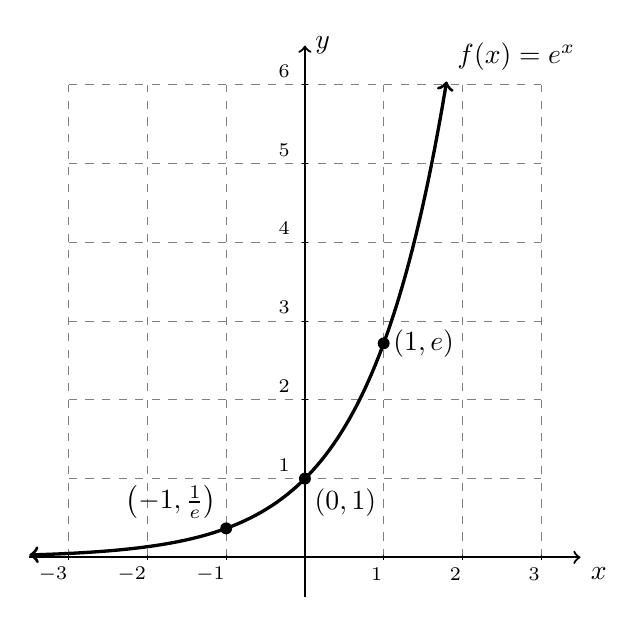
\begin{tikzpicture}[y=1.0cm, x=1.0cm,font=\sffamily]
    \begin{scope}
      %% ticks
      \draw[step = 1.0, gray,dashed] (-3,0) grid (3,6);
      %% axis
      \draw[thick,->] (-3.5,0) -- coordinate (x axis mid) (3.5,0) node[anchor = north west] {$x$};
      \draw[thick,->] (0,-0.5) -- coordinate (y axis mid) (0,6.5) node[anchor = west] {$y$};
      \foreach \y in {1,2,3,4,5,6} { \draw (1pt, \y) -- (-1pt, \y)
             node[font=\scriptsize,yshift=5,xshift=-1,anchor=east] {$\y$}; }
      \foreach \x in {-3,-2,-1,1,2,3} { \draw (\x,1pt) --
        (\x,-1pt) node[font=\scriptsize,yshift=-5,xshift=3,anchor=east] {$\x$};
      }

      \begin{scope}
        %% \clip(-4,-1) rectangle (8,5);
        \draw[scale=1.0,domain=-3.5:1.8,smooth,variable=\x,very thick,black,samples=100,<->]
             plot ({\x},{2.718^\x}) node[anchor=south west] {$f(x)=e^x$};

        \fill[black] (-1,0.368) circle [radius=0.5ex] node[anchor=south east,xshift=0]
             {$\left(-1,\frac{1}{e}\right)$};
        \fill[black] (0,1) circle [radius=0.5ex] node[anchor=north west,xshift=0]
             {$\left(0,1\right)$};
        \fill[black] (1,2.718) circle [radius=0.5ex] node[anchor=west,xshift=0]
             {$\left(1,e\right)$};

       \end{scope}
     \end{scope}

   \end{tikzpicture}




\subsection{Compound Interest} ~

\hspace{-.3in}
\begin{tabular}{ | p{0.9\textwidth} |} \hline 
  \noindent \underline{Compound Interest Formula (Annually, Monthly, Quarterly, Daily, Etc.)}  
  \begin{eqnarray*}
    A= P \left( 1+ \dfrac{r}{n} \right)^{nt}.
  \end{eqnarray*}
  In this formula, $P$ is the principal, $r$ is the annual interest rate in decimal form,
  $n$ is the number of interest periods per year, $t$ is the number of years $P$ is invested,
  and $A$ is the amount after $t$ years. \\ \hline
\end{tabular} 

\item Suppose \$2000.00 is invested at a rate of $3 \%$ compounded monthly. Find the \emph{principal after 18 months}. (Round your answer to the nearest cent.) \vfill


 \hspace{-.3in} \begin{tabular}{| l |} \hline
\underline{Continuously compounded interest formula} $A = Pe^{rt}$ \\
In this formula, $P$ is the principal, $r$ is the annual interest rate in decimal form, 
$t$ is the\\ number of years $P$ is invested, and
$A$ is the amount after $t$ years.   \\ \hline
\end{tabular}


\item If \$1500 is deposited in a savings account that pays interest at a rate of .1\% compounded continuously, find the balance after 7 years. \\[1in]


\newpage

\subsection{Exponential Functions in Applications} 
Increasing and decreasing exponential functions can be used in a
variety of real world applications.  For example:
\begin{itemize}
\item Population growth can often be modeled by an exponential function.
\item The growth of an investment under compound interest increases exponentially.
\item The mass of a radioactive substance decreases exponentially with time.
\end{itemize}

\noindent A substance that undergoes radioactive decay is said to be radioactive.  The \textbf{half-life} of a radioactive substance is the amount of time it takes for one-half of the original amount of the substance to change into something else.

\item The half-life of radium 226 is 1620 years.  In a sample originally having 1 gram of radium 226, the amount $A(t)$ in grams of radium 226 present after $t$ years is given by $\displaystyle A(t)=(\frac{1}{2})^{t/1620}$ where $t$ is the time in years after the start of the experiment.  How much radium will be present after 3240 years? 
\vfill


\end{enumerate}

\noindent \textbf{Student Learning Outcomes Check}

\begin{enumerate}
\item Can you recognize an exponential function graphically and algebraically?
\item Can you evaluate the exponential function base $e$?
\item Are you able to use exponential functions in compound interest and growth/decay problems?

\end{enumerate}

\noindent \textbf{If any of your answers were no, please ask about these topics in class.}

